\begin{frame}{Circuito 1: modelagem sem carga}
  \small
  \begin{columns}[T,onlytextwidth]
    \begin{column}{0.46\textwidth}
      \centering
      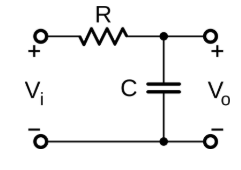
\includegraphics[width=0.65\linewidth,height=0.28\textheight,keepaspectratio]{slides/img/circuito_1.png}

      \begin{block}{Equação no domínio de Laplace}
        Com condições iniciais nulas,
        \[
          \frac{V_i-V_o}{R}=sCV_o.
        \]
        A saída é a tensão sobre o capacitor.
      \end{block}
    \end{column}
    \begin{column}{0.50\textwidth}
      \begin{alertblock}{Função de transferência}
        \[
          H_1(s)=\frac{V_o}{V_i}
          =\frac{Z_C}{R+Z_C}
          =\frac{1}{1+sRC}.
        \]
        \[
          K_1=H_1(0)=1,\qquad \tau_1=RC.
        \]
        \[
          p_1=-\frac{1}{RC},\qquad
          f_{c1}=\frac{1}{2\pi RC}.
        \]
      \end{alertblock}
      Em baixas frequências, $|H_1|\approx1$.
      Em altas frequências, a saída é atenuada.
    \end{column}
  \end{columns}
  \vspace{0.12cm}
  \centering\scriptsize
  Para uma fonte com resistência série $R_s$, o modelo referido à fonte ideal usa $R+R_s$.
  Nas medições, $V_i$ é obtido na entrada do filtro.
\end{frame}
